\chapter{Experiential Learning\\ of Networking Technologies}
\vskip -15pt

\centerline{{\LARGE\sl Evolution of Socket Programming – Part I}}

\vskip 0.8cm

\begin{center}
{\large\uppercase{Ram P. Rustagi}}, 

\vskip -6pt

Department of CSE, KSIT Bengaluru 


\bigskip
{\large\uppercase{Viraj Kumar,}} 

\vskip -6pt

Divecha Centre for Climate Change, IISc Bengaluru

\end{center}

\vskip 2.3cm



\vfill
\newpage

\begin{multicols}{2}

\section{Introduction}
 
 In the $21^{\rm st}$ century, the internet has become essential part of everyday tasks including banking, interacting with government services, education, entertainment, text/voice/video communication, etc. Individuals access the internet using client-side applications such as a browser or an app on their mobile phone or laptop/desktop. This client-side application communicates with a server-side application, typically running on a web server, which in turn may interact with other business applications. The underlying protocol is typically HTTP \cite{art1-key01} running on top of the TCP/IP protocol \cite{art1-key02}\cite{art1-key03}. A typical web server supports a large number (hundreds or thousands) of concurrent TCP connections. The most commonly deployed web servers in use today are Apache server \cite{art1-key04}, Nginx \cite{art1-key05}, or Microsoft Internet Information Server (IIS)\cite{art1-key06}. Nginx is mostly used on Linux and IIS runs only on Windows OS. In contrast, Apache web server (which is almost as old as the web itself) is supported on all platforms (Linux, Windows, MacOS, etc.). In its initial release in 1995 (version 1.3), Apache server could serve only a few concurrent clients, but its current release (2.4.41) can support a huge number of concurrent clients. In this article (as well as Part II that will follow), we will present a simplified view of this evolution that nevertheless explains how current web manage such high levels of concurrency. To do so, we will delve into socket programming, which is at the heart of managing TCP connections, and we will examine the key role that it plays in delivering high performance.

We have studied both transport layers protocol i.e., TCP \cite{art1-key02} and UDP \cite{art1-key07}, in detail in the last few articles, and we have developed a basic understanding of the working of the transport layer. This is a communication-enabling layer used by applications to exchange application-level data. Simple working of applications using TCP (providing reliable delivery) and UDP (providing best effort delivery) socket programming are provided in \cite{art1-key08}.  In this article, however, we will discuss increasingly complex levels of socket programming, from simple socket connections to complex connection management that are necessary to attain high TCP performance.  We will focus on TCP Socket programming only. UDP socket programming is simply a best effort delivery and socket implementation support does not impact the application communication performance. 

\section{Basis of TCP Socket Programming}

Any network-based application involves a pair of two programs, one that initiates the request and another one that receives the request and responds back. In normal parlance, these are correspondingly called the client and the server. For most practical purposes, these two entities reside on two different end systems and communicate with each other via an end-to-end logical network communication interface, called a socket. These two programs are most likely written by two different sets of developers and thus they need to follow an application protocol standard, such as HTTP, FTP, SMTP, etc.  These applications either run over TCP or UDP, a decision taken by the application developer. In this article, we will discuss the development of application program using TCP. We will start from very simple request/response communication and gradually increase complexity to involve multiple concurrent communications, sharing requests across many server processes with non-blocking socket communication to achieve performance gains. As before, we will have hands-on exercises where you will write and execute actual programs. Our example programs will be in the Python language, which is currently the most popular language (even though socket programming was originally written in C). These programs will explain the basics of socket programming and the various states of socket-enabling communication between the client and the server.

The client application initiates a TCP connection with the server using a \textit{TCP socket}. It communicates with the server through this socket, and finally closes the connection. To enable this bidirectional communication, the client first creates a socket (treated as file descriptor in the Unix system) and connects it to the server by specifying the server’s address (IP address and TCP port number). The server must have created a socket beforehand to enable this connection i.e., it must be ready to accept connections from clients. This connection setup involves a 3-way TCP handshake \cite{art1-key09}\cite{art1-key10}\cite{art1-key11} which remains transparent to the client and server applications. This is followed by data transfer in TCP\break ESTABLISHED state \cite{art1-key11}. Finally, the connection closure involves a handshake of four messages \cite{art1-key12}, which again remains transparent to applications. The interaction of client and server programs with the network is implemented using socket library API calls. In this article, we first discuss the usage of these API calls in a simple way. We will enhance the complexity later to improve server performance.

\section{Socket Programming Approaches}

An introduction to socket programming is given in \cite{art1-key09}\cite{art1-key13}\cite{art1-key15}, and brief description of each API call can be found at \cite{art1-key14} and from the man pages \cite{art1-key16}.  The most common understanding of a simple client-server interaction is shown in Figure~\ref{fig01} \cite{art1-key11} and elsewhere in the networking literature. At first, the server creates a socket using \textit{socket()}, binds this socket to a well-known address (IP address and port number) using \textit{bind()}, informs the TCP stack of the underlying Operating System about the number of connections that can be in queue waiting to be served by the server using \textit{listen()}, and then accepts one connection at a time using \textit{accept()}. For reasons that will become clear soon, let us understand these API calls through the following analogy. Suppose several students (client applications) want to communicate with their college principal (server application) in his/her office. The \textit{socket()} call is analogous to the principal’s secretary opening the office prior to the principal’s arrival. The \textit{bind()} call is analogous to the principal entering the office, although s/he is still not available to communicate with students. After a while, the principal allows students to enter the waiting room, which is analogous to the \textit{listen()} call. The number of chairs in the waiting hall corresponds to the size of the TCP listen queue. If there are $N$ chairs in the waiting hall, at most $N$ students can wait. If there are $M$ students (where $M > N$), then the secretary must turn away $M – N$ students.

\begin{figure}[H]
\centering

\includegraphics[scale=2.3]{src/Figures/chap1/fig01.jpg}
\caption{Typical understanding of client server interaction}\label{fig01}

\vspace{-.4cm}

\end{figure}

When principal is ready to meet students, the secretary allows one student into the office. This is analogous to the \textit{accept()} call. Typically, the secretary will send students in a first-come first-served (FCFS) manner, although this is not necessary. Analogously, the TCP stack may or may not implement a FCFS policy. (When the student enters, there is a vacancy in the waiting room and another student may now occupy this space.) The student in the office now communicates with the principal, analogous to a series of \textit{read()}/\textit{write()} calls. The principal may permit multiple students to enter the office – this is analogous to the server issuing a series of \textit{accept()} calls and communicating concurrently with multiple clients. Just as the number of students simultaneously within the principal’s office bears no correlation to the number of students waiting outside, the number of concurrent communications is independent of the number of clients waiting in the TCP listen queue. In brief, a TCP server application follows the path sequence \textit{bind()}, \textit{listen()}, and \textit{accept()} socket API calls, followed by needed number of \textit{read()}/\textit{write()} calls. 

The client-application follows a somewhat different path of socket API calls. It first creates a socket (its endpoint of communication) using the \textit{socket()} call. For a client to be able to talk to server, it must know IP address and port number of server application. The client provides these two parameters (IP address, port number) as part of the \textit{connect()} call to establish communication with the server. The invocation of \textit{connect()} initiates the 3-way TCP handshake. Once the connection is established, the client follows a series of \textit{write()}/\textit{read()} call to send data to and receive data from the server. Finally, the client closes the TCP connection.

\begin{figure}[H]
\centering
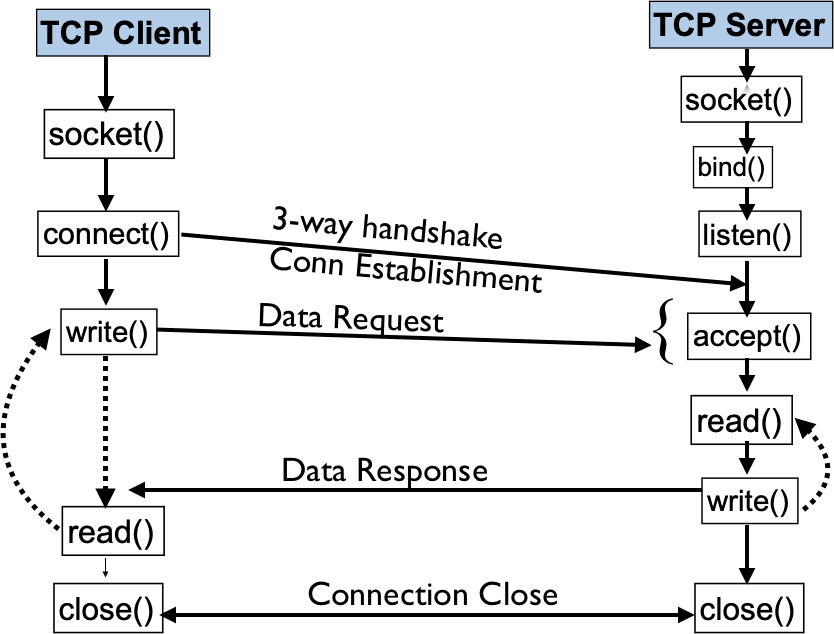
\includegraphics[scale=2.3]{src/Figures/chap1/fig02.jpg}
\caption{Practical working of TCP sockets interaction}\label{fig02}

\vspace{-.4cm}

\end{figure}

The communication flow in Figure~\ref{fig01} provides a common conceptual understanding of TCP client-server interaction typically followed for TCP-based communication, with the 3-way handshake performed after the server issues the \textit{accept()} call. In actual implementations of the TCP stack, the communication flow for the server is slightly different as shown in Figure~\ref{fig02}. Let us understand this difference using our earlier analogy of students and the college principal. When a student enters the waiting room, s/he is ready to communicate with the principal - this is analogous to the client application making a \textit{connect()} call. Taking the analogy one step further, the student can start filling out necessary paperwork while waiting even though the principal has not yet invited the student to enter. This is analogous to the client application invoking a \textit{write()} call and sending data to the server, even though the server has not yet invoked the \textit{accept()} call. Thus, the key difference between\break Figure~\ref{fig01} and Figure~\ref{fig02} is that the client can invoke \textit{connect()} to establish communication with the server as soon as the server invokes \textit{listen()}. From the client application’s perspective, the connection is successful - it can and even begin to send data to the server on the assumption that the server application will invoke the \textit{accept()} sometime later and read the data sent to it (as shown in Figure~\ref{fig02}). Note that there is no guarantee that the server application \textit{will} issue an \textit{accept()} call - the server may crash, for instance - but the client assumes that this will not happen. In the discussion below, we will study this behavior of the server-side TCP connection management with respect to multiple concurrent clients and explore the functionality of socket APIs.

\vspace{-.5cm}

\section{A Server with Just One Client\\ Connection}

A very simple TCP server program would correspond to accepting requests from only a single client, serve these requests and then exiting. We can use \texttt{netcat} as a server \texttt{(nc -1 <port>)} for this simple communication. This command runs a TCP server binding on the specified port with option \texttt{-1} and all the IP addresses associated with the server machine. The netcat server accepts a single client request. As long as the client is connected, the server will receive messages from the client and display these on its terminal window. When the client closes the connection, this simple server closes the connection as well and exits. However, to develop a better understanding of using \textit{bind()}, \textit{listen()} and \textit{accept()} calls, consider a simple Python program \texttt{tcp\_server01.py} \cite{art1-key17}. The required code snippet is shown in the left column of Table~\ref{tab01}. The invocation of socket APIs \textit{bind()}, \textit{listen()} and \textit{accept()} are respectively shown on lines 3, 5 and 7. The server reads the client’s requests (lines 9 to 13). The detection of connection closure by the client occurs when the reading of data fails (i.e., it returns NULL) on lines 11-12. When this occurs, the server program comes out of its perpetual loop, closes the connection (line 14) and exits (line 15). This code is very similar in behaviour to netcat \texttt{(nc)} server. By default, in all our exercises we will use \texttt{netcat (nc)} as the simple TCP client program which will be invoked as \textbf{“nc <server IP> <server port>”}, unless specified otherwise.
\end{multicols}

\setcounter{section}{0}
\begin{table}[H]

\vspace{-.8cm}

\centering
\caption{Server program that accepts 1 client request}\label{tab01}
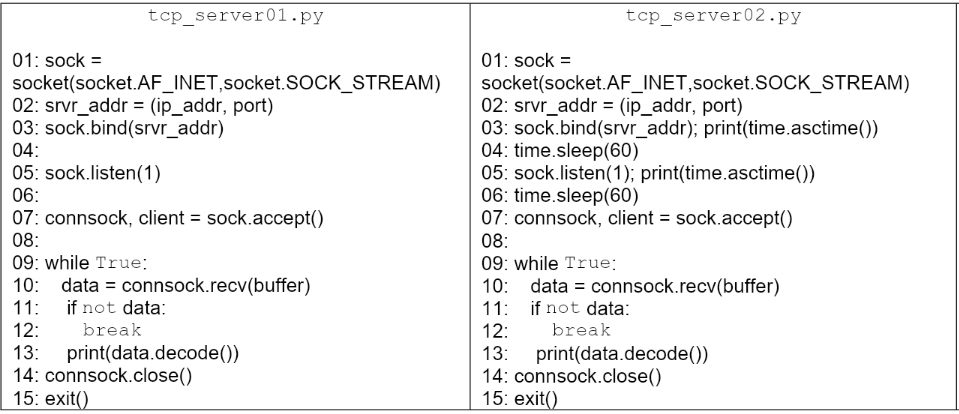
\includegraphics[scale=2.25]{src/Figures/chap1/tab01.jpg}
\end{table}

\vspace{-.6cm}

\begin{multicols}{2}
To understand interdependencies between \textit{bind()}, \textit{listen()} and \textit{accept()}, consider the code snippets of its modified version in program \texttt{tcp\_server02.py} \cite{art1-key17} as shown in the right column of Table~\ref{tab01}. The server invokes \textit{listen()} (line 5) 60 seconds (line 4) after its binds (line 3) to its port number. So, when program starts running, for the first 60 seconds, the TCP stack/OS on the server machine has no information if the server program will receive and serve any client requests and if any clients can be put into the waiting queue. Thus, until the time \textit{listen()} is invoked by the server (line 5), if a client tries to connect to the server, the connection attempt will be unsuccessful. To see this behaviour, an example invocation is shown in right column of Table~\ref{tab02}. The server program by default uses TCP port number 9999 (this can be changed using the option \texttt{-p}), and is started at \texttt{08:59:29} as shown by the $2^{\rm nd}$/$3^{\rm rd}$ lines in right column of Table~\ref{tab02}. The \texttt{netcat (nc)} program \cite{art1-key18} is used as a client to connect to this server, and its invocation is shown in the left column of Table~\ref{tab02}. The first two connection attempts at times \texttt{08:59:37} and \texttt{09:00:18} are terminated as the server program hasn’t yet executed the \textit{listen()} call. The status of at server side shows no connection until time \texttt{09:00:30} (shown in lines 1-4 in Table~\ref{tab03}). The \textit{listen()} API (line 5 in the right column of Table~\ref{tab01}) is invoked at time \texttt{09:00:29} (line 4 in right column of Table~\ref{tab02}). The next client connection attempt after \texttt{09:00:29} (i.e., at time \texttt{09:00:36}) is successful (lines 5-8 in the left column of Table~\ref{tab02}). Lines 5-7 of\break Table~\ref{tab03} show that the server is ready to listen for client\break connections.
\end{multicols}

\begin{table}[H]

\vspace{-.7cm}

\centering
\caption{Network implication of delayed \textit{listen()}, \textit{accept()}}\label{tab02}
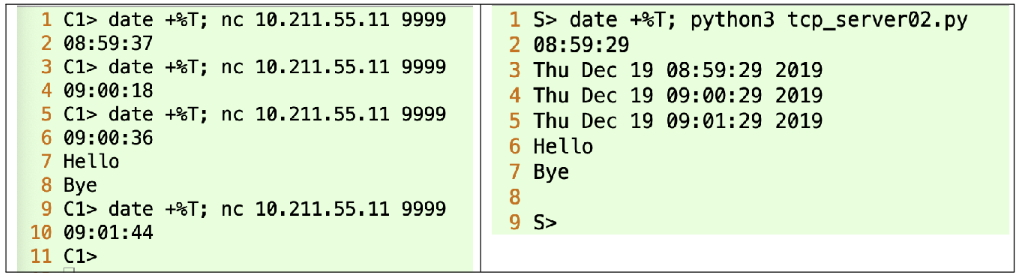
\includegraphics[scale=2.15]{src/Figures/chap1/tab02.jpg}
\end{table}

\begin{table}[H]

\vspace{-.7cm}

\centering
\caption{Status of network connection at Server Machine}\label{tab03}
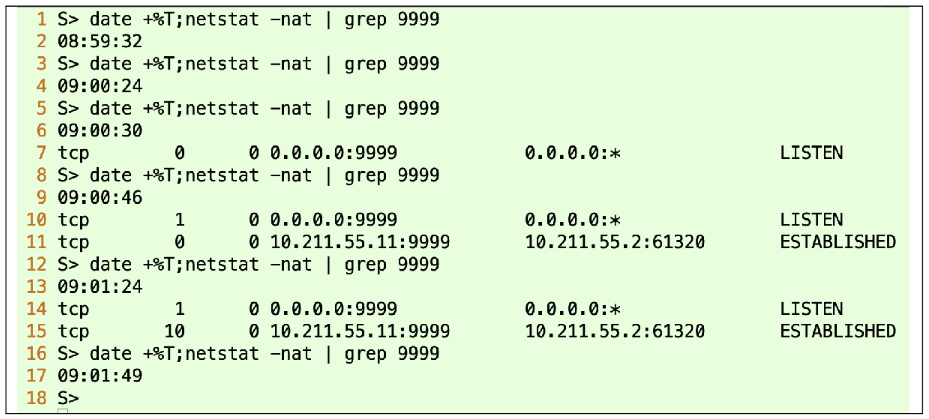
\includegraphics[scale=2.35]{src/Figures/chap1/tab03.jpg}
\end{table}

\begin{multicols}{2}
At this stage, the server program is still waiting for 60 seconds (line 6 in the right column Table~\ref{tab01}), and it has not accepted the client connection yet. The server program invokes \textit{accept()} (line 7 right column of Table~\ref{tab01}) at time \texttt{09:01:29} and accepts the connection only then. However, from the client’s perspective, the TCP connection is established at time \texttt{09:00:36} as shown by lines 8-11 in Table~\ref{tab03}. Since the connection is established from the client’s view, the client can send data on this connection as shown by lines 5-6 in client’s window (left column of Table~\ref{tab02}). This data ( \texttt{“Hello + $\backslash$n + Bye + $\backslash$n”} ; a total of 10 characters) has reached the server and is in the queue of this connection at the server side as shown by value of the second field (line 15 in Table~\ref{tab03}). The data remains in the queue till \texttt{09:01:29}, at which time server accepts the connection. The server program accepts the client connection by invoking \textit{accept()} at time \texttt{09:01:29} (line 5 in right column of Table~\ref{tab02}). After it reads the data, the queue for this connection is cleared. When the client exits at time \texttt{09:01:44}, the connection is closed on the server side as well and the network connection status shows no connection at time \texttt{09:01:49} (lines 16-17 in\break Table~\ref{tab03}).

In general, a server program should be able to serve multiple clients. Thus, whenever one client connection closes, it should accept a request from the next waiting client, if any, and so on. The number of clients that can remain in the queue is determined by the parameter value of the \textit{listen()} call. If a new client connects when the queue is full, this connection request is rejected and the client program would exit after a certain number of retries. To study the impact of queue size, run the server program \texttt{tcp\_server02.py} \cite{art1-key17} again and connect to this server with multiple client programs. When the listen queue becomes full, the TCP stack\break implementation on the server machine simply ignores TCP SYN (connection setup request \cite{art1-key09}\cite{art1-key11}) and does not respond at all. The client will retry the connection by resending TCP SYN packets - the number of times is pre-configured and is identified by the system configuration and tuning parameter \texttt{net.ipv4.tcp\_syn\_retries} (the default value is 6 on Ubuntu Linux). As per the TCP timeout implementation, each time it sees a timeout, it doubles the timeout value \cite{art1-key09} and retransmits the packet again. For our purpose of studying the listen queue size behaviour, it is recommended to set this configuration parameter to the smallest positive integer value of \texttt{1}. On a Linux machine, use the command \texttt{sudo sysctl -w net.ipv4.tcp\_syn\_retries=1}. Further, as per the Linux system implementation of the \textit{listen()} socket call \cite{art1-key18}, the real maximum queue length is 1.5 times the parameter value passed in the \textit{listen()} API. In our example, the server program invokes \textit{listen(1)}, the queue size is expected to be 1.5, and thus the observed value is 2. This implies that at any point in time, there will be at most 2 clients in the TCP queue waiting for server to accept the connection.
\end{multicols}

\begin{table}[H]

\vspace{-.9cm}

\centering
\caption{Concurrent client requests to a single server}\label{tab04}
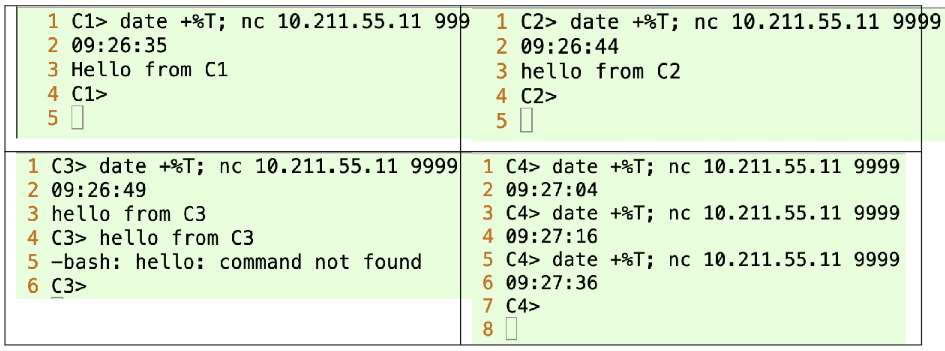
\includegraphics[scale=2.28]{src/Figures/chap1/tab04.jpg}
\end{table}

\begin{table}[H]
\centering

\vspace{-.8cm}

\caption{Single request handling Server connection status}\label{tab05}
\smallskip
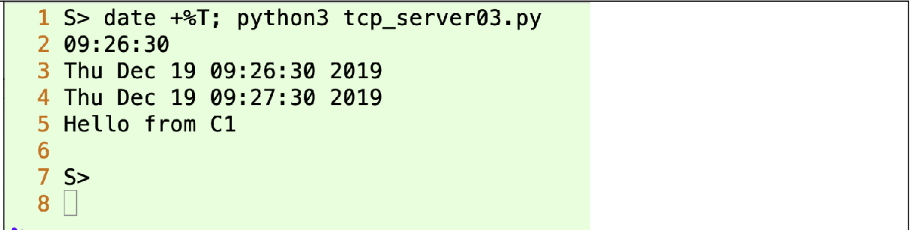
\includegraphics[scale=2.35]{src/Figures/chap1/tab05.jpg}
\end{table}

\begin{multicols}{2}
To study the behaviour of \textit{listen()} and backlog of queues in an efficient manner, the server program is modified just to put a delay of 60 seconds between \textit{listen()} and \textit{accept()}. There is no need to have any delay between \textit{bind()} and \textit{listen()}. The invocation of this new server program \textit{tcp\_server03.py} is shown in Line 1 of Table~\ref{tab05}. We invoke 3+ clients to connect to it (with \texttt{syn\_retries} value set to 1 on the client machine) within 60 seconds of starting of the server program. This should result in the first two clients connecting successfully to the server (actually these should be in TCP connection queue) and the third client program should be unsuccessful after retries. The server program \texttt{tcp\_server03.py} \cite{art1-key17} starts at time \texttt{09:26:30} (line 2 of Table~\ref{tab05}), invokes \textit{bind()} and \textit{listen()} at the same time (line 3 of Table~\ref{tab05}) but waits for 60 seconds before executing \textit{accept()}. The invocation of client programs \texttt{(nc)} is shown in Table~\ref{tab04}, where client C1 starts at time \texttt{09:26:35} and client C2 starts at time \texttt{09:26:44}. These clients connect successfully, as shown in the top row of Table~\ref{tab04}, whereas client C3 starting at time \texttt{09:26:49} and client C4 starting at time \texttt{09:27:04} (shown in the bottom row of Table~\ref{tab04}) are unsuccessful in connecting because these two are invoked within 60 seconds of starting of the server program where the server queue has become full, corresponding to a listen queue size being 1. The input \texttt{‘hello from C3’} shown for client C3 does not act as input to this client program, but instead becomes a Bash shell command when C3 exits - this is an unknown command, and hence the Bash shell gives error \texttt{‘hello: command not found’} (lines 4-5 bottom row of left column of Table ~\ref{tab04}). The TCP server shows two connections in the ESTABLISHED state (lines 1-13 of\break Table~\ref{tab06}) during the time from \texttt{09:26:32} to \texttt{09:27:08} - note that both these are before the time 09:27:49, when the server invokes \textit{accept()}.
\end{multicols}

\begin{table}[H]

\vspace{-.9cm}

\centering
\caption{Connection Queue status before/after \textit{accept()}}\label{tab06}
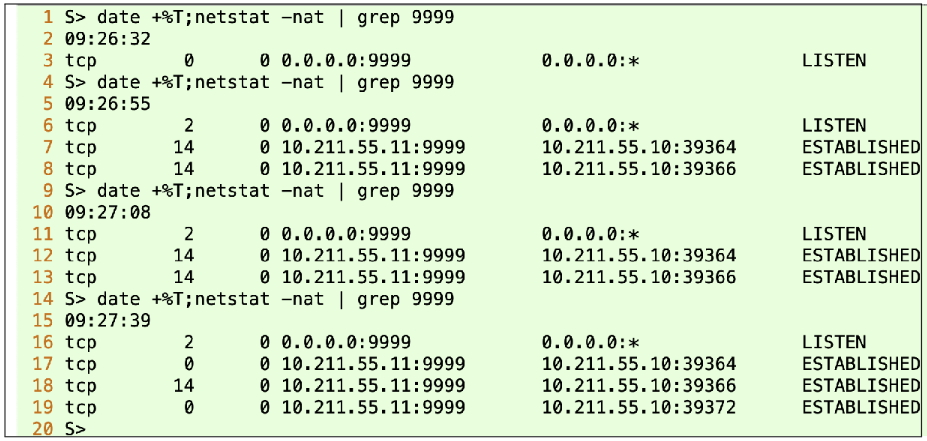
\includegraphics[scale=2.35]{src/Figures/chap1/tab06.jpg}
\end{table}

\begin{table}[H]

\vspace{-.7cm}
\centering
\caption{TCP SYN Retries on listen Q full}\label{tab07}
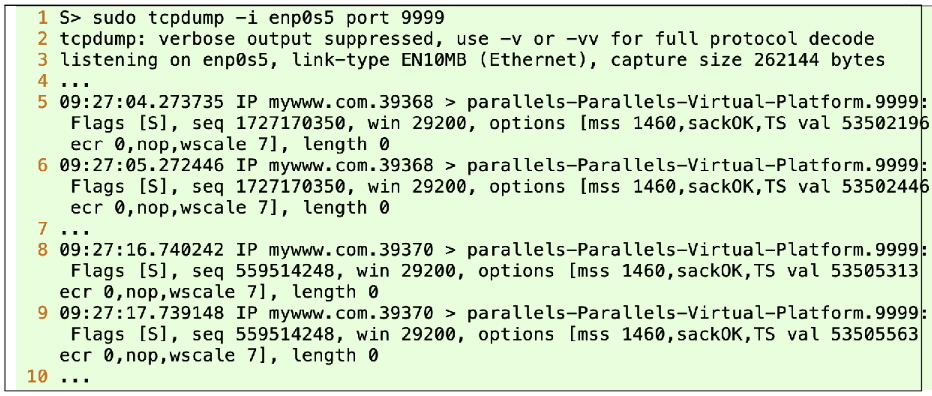
\includegraphics[scale=2.35]{src/Figures/chap1/tab07.jpg}
\end{table}

\vspace{-.6cm}

\begin{multicols}{2}

At time \texttt{09:27:30}, the server program invokes \textit{accept()} (line 4 Table~\ref{tab05}). When a new client connects after this time (invocation of C3 is not shown in the table), this client connects successfully and the number of connections in the ESTABLISHED state becomes 3 as shown in lines 14-19 of Table~\ref{tab06}. Line 16 of Table~\ref{tab06} shows the size of the listen queue as 2, corresponding to two connections (C2 and C3) pending to be accepted, and line 18 shows the queue size to be 14 implying that a client has sent 14 bytes of data (this corresponds to \texttt{hello from C2$\backslash$n}) which needs to be read by the server. When the $4^{\rm th}$ client, shown in lines 5-6 in the bottom row of the right column of Table~\ref{tab04}, tries to connect at time \texttt{09:27:36}, the connection fails since the server connection queue is already full on account of clients C2 and C3. Table~\ref{tab07} shows the excerpts of \texttt{tcpdump} output, which demonstrates that two TCP SYN packets are received. The second SYN packet corresponds to TCP retransmit. Lines 5-6 correspond to the first connection request at time \texttt{09:27:04}, and lines 8-9 correspond to the second connection request at time \texttt{09:27:16}. No response is given by the server as these TCP SYN connection requests are ignored because TCP listen queue is full.

When the first client exits (by pressing Ctrl-D in \texttt{nc}), the connection is closed and the server also exits after serving one client. This is because the server program \texttt{(tcp\_server03.py)} accepts only one connection, and exits after this first connection is closed. The connection from the other two clients (C2, C3) are simply terminated without any actual connection accepted nor received data read by the server. From the client’s perspective, this is a bit puzzling since the client initially sees that the connection is in the ESTABLISHED state. However, the client has no clue why the connection was terminated.

\setcounter{section}{4}
\section{A Perpetual Server with Just One Client Connection at a time}

In general, a server program is expected to run for ever, and thus a natural extension to the server program \texttt{tcp\_server03.py} is to accept new client requests after its interaction with the currently connected client is over. This requires that the server program should be in perpetual running loop that would accept a new connection, service the client and then go back to accept next connection from the new client. A sample snippet of such a code from server program \texttt{tcp\_server04.py} \cite{art1-key17} is shown in Table~\ref{tab08}. The perpetual loop starts at line 5, whereas serving of individual client requests is handled in lines 6-13.

This server program works fine in dealing with any number of clients. However, such a server suffers from severe performance issues. Since the sever is handling one client at time, all other clients in the queue have to wait for earlier clients before they get any service. Such a response is unacceptable in real-life situations. Consider a bank website that works in this way i.e., it serves only customer login and associated interactions one at time. All other customers who are waiting in the queue will get totally frustrated and would not use the bank website again at all. Thus, for an effective web server, it is of paramount importance to serve the multiple clients concurrently.
\end{multicols}

\begin{table}[H]

\vspace{-.6cm}

\centering
\caption{Perpetual server with one connection at a time}\label{tab08}
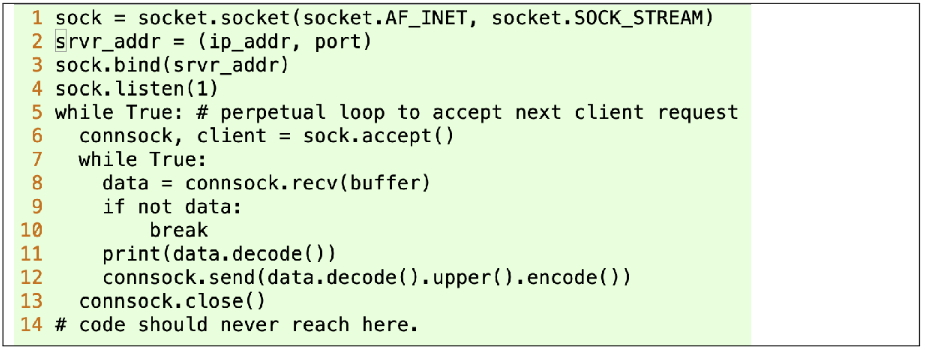
\includegraphics[scale=2.35]{src/Figures/chap1/tab08.jpg}
\end{table}

\begin{multicols}{2}

\vspace{-.17cm}

\section{A Perpetual Server with Multiple Concurrent Connections}

Modern webservers (e.g., Apache \cite{art1-key04} and Nginx \cite{art1-key05}) can serve hundreds of thousands of concurrent clients. These web servers provide a lot more functionality than just managing concurrent TCP connections and have evolved into complex implementations with many supported features to serve these clients efficiently. In this article, we will take a simplistic view from the TCP perspective to see how these concurrent clients are served. There are several design/implementation choices to serve multiple concurrent clients, and we will start from a very simple approach and progress towards more complex implementations to demonstrate efficiency improvements.

The most simplistic approach to serve many clients concurrently is to have one main server process that acts as a parent process and creates a separate child process per client. Thus, a parent process starts and waits for new client request. Whenever a client connects, it spawns a new child process dedicated to serving the client. Once the client closes the connection, this child process exits. A simple code snippet of such a simplistic server program \texttt{tcp\_server05.py} \cite{art1-key17} using this approach is shown in Table~\ref{tab09}.

\end{multicols}

\begin{table}[H]

\vspace{-.8cm}

\centering
\caption{Server spawning child process for each client}\label{tab09}
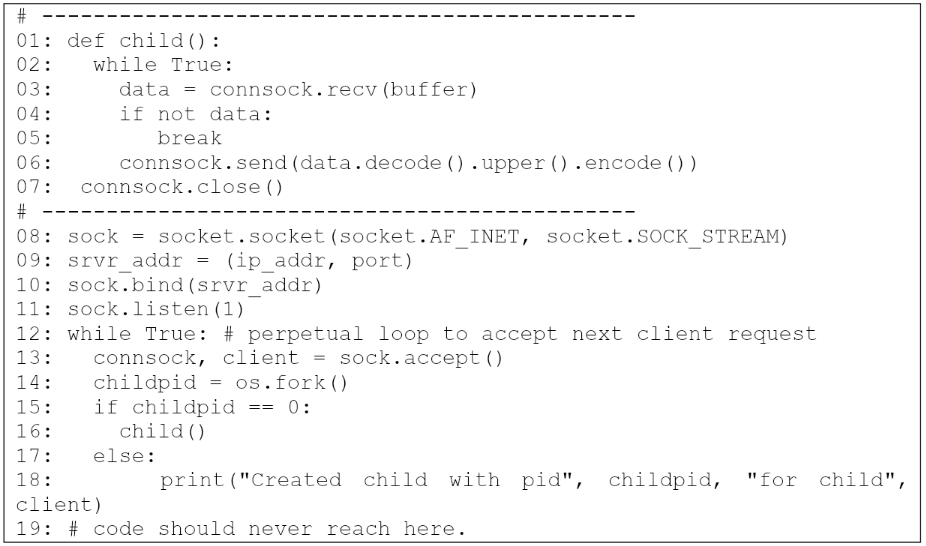
\includegraphics[scale=2.35]{src/Figures/chap1/tab09.jpg}
\end{table}

\begin{table}[H]

\vspace{-.8cm}

\centering
\caption{Modified sever code waiting for child to exit}\label{tab10}
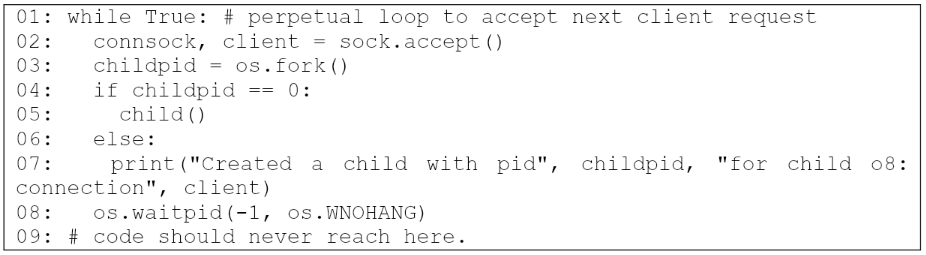
\includegraphics[scale=2.35]{src/Figures/chap1/tab10.jpg}
\end{table}

\begin{multicols}{2}

\vspace{-.7cm}

The inefficiency of this approach lies in the fact that a new process needs to be created (lines 13-14 of Table~\ref{tab09}) for each client. Creating a new process consumes significant amount of OS resources, both in terms of memory and compute time. This approach can work well for a limited number of concurrent clients - a few hundred or possibly a thousand. But when the number of concurrent clients increases, the process scheduling by the operating system itself will take a heavy toll on the system performance and bring down the system. Thus, this approach is not scalable. Another common problem that developers often face in this approach corresponds to zombie or defunct processes. This problem arises when a child process exits, but the parent does not wait for the exit status of a child process. As per Unix process implementation, a parent must wait for the child process to exit, receive the exit status of the child process and take necessary action (which in most cases is none). A child process which has exited and is waiting for its parent to receive its exit status is known as zombie process. Although zombie processes remain idle and do not consume CPU time, they nevertheless consume process table resources of the underlying operating system. So, if such a server application has been running for some time and has received $N$ new client connections, there will be $N$ zombie processes in the system when these clients exit. For some large $N$, the system will run out of resources (process table memory space). A simple solution to resolve this issue is that the parent must invoke the \textit{waitpid()} method for the exited child process. A sample snippet of modified server program \texttt{tcp\_server05b.py} \cite{art1-key17} which invokes \textit{waitpid()} is shown in Table~\ref{tab10}. The method \texttt{waitpid()} is invoked with two parameters. The first parameter corresponds to process id of child process (\texttt{-1} implies any child), and the second parameter \texttt{WNOHANG} implies that this method is non-blocking. If a child has exited, this method will return the exit status of that child. Otherwise, it will return error (-1) but it will not wait for the child to exit.
\end{multicols}

\begin{table}[H]

\vspace{-.3cm}

\centering
\caption{server creating predefined number of child processes}\label{tab11}
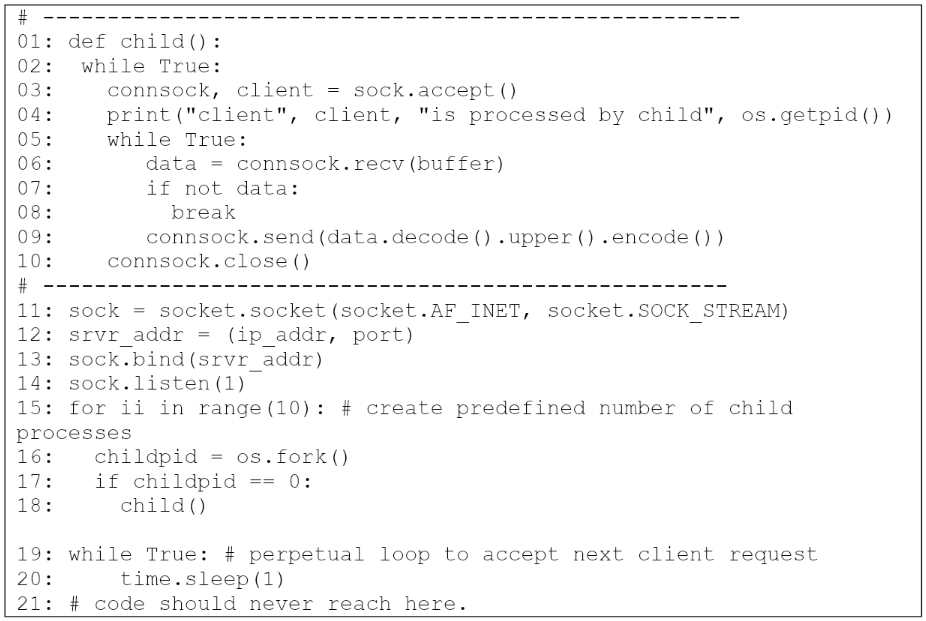
\includegraphics[scale=2.35]{src/Figures/chap1/tab11.jpg}
\end{table}


\begin{multicols}{2}

One possibly way to improve the performance efficiency of this approach would be to avoid creating a child process every time a new client connects. Instead, we could pre-create a fix number of children processes beforehand and assign new client connection requests to any of the free children processes. The sample snippet code of a server program \texttt{tcp\_server06.py} \cite{art1-key17} implementing this approach is shown in Table~\ref{tab11}.  This code snippet pre-creates 10 children processes as shown in lines 15-16  \texttt{‘for ii in range(10):’} when the server starts. The parent process remains idle for all practical purposes. Each child process invokes its own \textit{accept()} and it is up to the OS to pick any of the child process waiting on \textit{accept()} and assign the new incoming connection request to it. Thus, the approach of distributing the new connections has also been moved from the user space to the kernel space. This approach certainly helps enormously in saving the OS overhead of creating a process, and thus performs better than the earlier approach of creating a new child process upon arrival of each new client connection request.

However, this approach poses a new problem which can significantly impact the server process performance. When the number of clients exceeds the total number of pre-created children processes plus the required queue size, then those clients will be denied connection requests from the server. A simple solution to address this issue would be that each client communicates its current connection status to the parent. Whenever the child process receives a new client request, or when the connection is closed, it informs the parent process. This requires a separate channel of communication between all clients and the server, leading to additional complexity of implementation. The parent keeps track of the number of clients currently being served. Thus, when it sees that the number of connected clients is approaching the number of pre-created children processes, it pre-creates more children processes. Similarly, when number of free children processes exceeds a specified threshold, it can abort a certain number of idle children processes and thus make efficient use of the server’s system resources. This entails some amount of communication between children and parent process, and it requires the parent process to do some book-keeping to dynamically create/kill child processes. A further improvement can be done by using threads instead of creating child processes. This way, OS scheduling overhead is lower compared to dealing with separate child processes. Although threads are more efficient than child processes, writing a thread-safe code is yet another challenge that developers need to deal - not many programmers can write efficient, robust multi-threaded code. However, the problem of scaling still persists and only a limited number of clients can be served using these approaches. 
\end{multicols}

\begin{table}[H]
\centering
\caption{Concurrent connections handling using \textit{select()} call}\label{tab12}
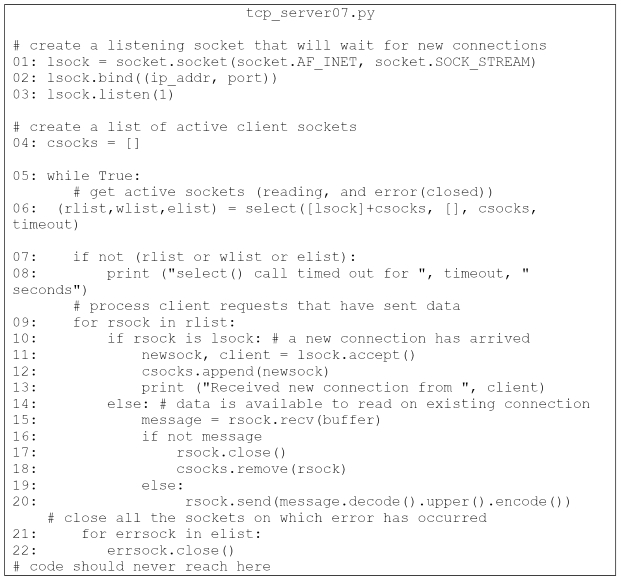
\includegraphics[scale=3.5]{src/Figures/chap1/tab12.jpg}
\end{table}


\begin{multicols}{2}
\section{Serving Multiple Concurrent\\ Connections using \textit{select()}}

For an efficient server process implementation, it is desirable not to dedicate one child process for each new client, and to avoid pre-forked approach of creating a specified number of children processes or dynamically creating children processes. However, the server program must concurrently handle multiple clients. In general, when $N$ clients are connected to the server, not all of them communicate with server at the same time and any design approach should keep this in mind. For example, consider $N$ browsers accessing a web server. When a web page is downloaded, a user will take some time to glance over (read) it, and there will be significant time gap before the next request is made from this browser to the web server. Thus, at any point of time, only a few clients would concurrently send request data to the web server and be waiting to receive responses. A naïve approach to efficiently deal with this situation is a single threaded process, where it maintains all the connected socket in an array data structure and continuously checks which of the client socket in the array has received the request data from the associated client and respond accordingly. The socket library call \textit{select()} (C language: \cite{art1-key20}, Python 3 documentation: \cite{art1-key21}) provides exactly this functionality. The method accepts a list of all open sockets as inputs. Upon invocation of \textit{select()}, it checks which of the sockets in the input list have data availability, and it returns back a list of only the active sockets to the server application. For each of these active sockets (i.e., clients which have sent data), the server program reads the data and communicates accordingly. The original listening socket on which new connections arrive is also a part of the input list of sockets. Whenever a new client connects, this listening socket activity is considered at par with read and needs to be checked for accordingly. The server program using the \textit{select()} API call is given in \texttt{tcp\_server07.py} \cite{art1-key17} and the key code snippet is shown in Table~\ref{tab12}.

The server program \texttt{tcp\_server07.py} is a simplified example of handling concurrent client connections. It is limited to reading data from client requests only and it does not show the use of \textit{select()} API for writing data on these sockets. The \textit{select()} method (in Python) requires 4 parameters:

\vspace{-.5cm}

\begin{itemize}

\setlength{\parskip}{0pt}
  \setlength{\itemsep}{0pt plus 6pt}

\item[\rm a.] List of sockets on which data can be sent by clients,

\item[\rm b.] List of sockets where data can be written, but given empty list in this example,

\item[\rm c.] List of sockets which have been closed by the \textit{clients()}, and

\item[\rm d.] Timeout value.

\end{itemize}

This timeout is used for \textit{select()} call to return if no active sockets are found from these 3 lists. New arriving connection processing is shown in lines 10-13. The processing of request data from active clients is shown in lines 14-15, 19-20. Lines 16-18 show the connection processing when the client closes the connection.

The approach of using \textit{select()} performs better than earlier approaches of creating multiple threads/processes. The \textit{select()} call is based on a Unix system call \cite{art1-key19}\cite{art1-key20}, which in general has a default limit of 1024 connections as this is internally based on a 1024-bit vector implementation. Thus, a server using \textit{select()} is generally limited to handling 1024 concurrent clients. Modern servers need to deal with many more than 1024 concurrent connections, and thus \textit{select()} is insufficient for this purpose. This limit of 1024 concurrent clients is overcome by two other socket API calls, namely \textit{poll()} and \textit{epoll()}, which we will discuss in our next article. The major difference between \textit{poll()} and \textit{select()} corresponds to internal implementation details, and the former is more efficient than latter. Further, \textit{poll()} supports more than 1024 clients as well. Socket API \textit{epoll()} is an event based implementation and is much more efficient than \textit{poll()} in terms of performance.

\section{Summary}

We have discussed the progression of approaches for a TCP server program to handle multiple concurrent clients. The simplest server processing starts from processing one client at a time. This causes significant delays to waiting clients, leading to a poor user experience. The next approach is to create one server child process (or thread for more efficient processing) per new client, which is a simplified and robust approach as each child process separately deals with each client. This makes the programming simple, as the developer does not have to write code for managing multiple sockets. This approach works fine but it is highly inefficient since creation of child process results in high overhead for the underlying OS. Another alternative is to create a pre-configured number of children processes (or threads). This avoids the overhead of process creation at run-time but it imposes a limit on the number of concurrent clients that can be served. The next approach is to use a mix of pre-creating a fixed number of children processes and then dynamically adjusting the number of children depending upon the number of clients connected. A better and more efficient approach that overcome the known limitations is to make use of the \textit{select()} API to serve multiple concurrent client. This again has some efficiency issues and generally has a limit on number of 1024 concurrent clients (this can be changed by recompiling the Linux kernel). More efficient processing is provided by use of \textit{poll()} and \textit{epoll()} calls, to be explored in the next follow up article.

A practical example of understanding the progression of server-side programming using the above discussed approaches can be seen in the implementation of the popular cross platform Apache web server \cite{art1-key04}. The web server supports a \textit{pre-forked} model where a number of preconfigured children processes are created. The parent process manages the size of server pool and creates or kills child processes as required. The web server also supports a \textit{worker} model where the child process creates multiple threads to process multiple clients. This is more efficient than \textit{pre-forked} approach. Finally, the most efficient supported implementation corresponds to \textit{event} model, which implements a hybrid multi-process, multi-threaded server. This consumes less resources compared to worker model. The event model of Apache web server is supported on Unix variants but not on Windows. Another, widely deployed web server is Nginx \cite{art1-key05} which by default is a single threaded server (per CPU core). It basically creates one child process for each CPU core in the system and thus number of children processes remains independent of number of clients connecting to it. It also provides a more efficient implementation using the \textit{epoll()} mechanism.

\vspace{-.3cm}

\section{Experiential Exercises}

\vspace{-.2cm}

The complete code of server programs as discussed in the article for both Python and C language (not shown in the article) can be accessed from \cite{art1-key17}. The experimental setup for these exercises consists of a simple setup of two machines connected on a network, one acting as a client and other server. The server machine should be running Linux operating systems, whereas client could be Linux, MacOS or Windows, but preferably Linux. For the client application, \texttt{netcat (nc)} \cite{art1-key18} would be used, which is available by default on Linux and MacOS, but need to be installed (Free and open source version available on Internet) on Windows OS. On the server machine, Python scripts would be invoked. As a place holder, the IP Address of client and server are respectively taken as 10.211.55.2/24 (some examples may show the client address as 10.211.55.9/24) and 10.211.55.11/24. The server programs \texttt{tcp\_server<NN>.py}, by default, uses the port number 9999 and can be invoked with any other value using option -p. On the client machine, configure the number of SYN retries to 1. On Linux based clients, this can be done by changing system TCP SYS retry attempts e.g. \texttt{sudo sysctl -w  net.ipv4.tcp\_syn\_retries=1}.

\vspace{-.3cm}

\setcounter{section}{0}
\section*{Exercise \thnum{1}\label{chap1-exe01}}

\vspace{-.2cm}

\textbf{Topic: TCP Server handling a single client with\\ multiple clients queueing.}

\vspace{-.2cm}

\begin{itemize}
\item[a.] Invoke the server program \texttt{tcp\_server01.py} on server machine. This server accepts only one client request and exits after client closes the connection.

\item[b.] On the client machine(s) [can use more than 1 client machine as well], invoke netcat in 3 different terminal windows as below

\texttt{nc 10.211.55.11 9999}

\item[c.] All 3 clients would be connected. From each of the client send some data e.g. \texttt{“Hello 1”, “Hello 2”, “Hello 3”,} etc.

\item[d.] On the server, check connection status as below.

\texttt{Netstat -natp | grep 9999}

\item[e.] It should show 3 connections in ESTABLISHED state similar to that shown in Table~\ref{tab06}. The data sent from first client will be shown on server terminal, data from other two clients will be shown as queued in $2^{\rm nd}$ column of \texttt{netstat} output.

\item[f.] Exit from the first client. Check the connection state on the server. All 3 connections would be closed and server program would also exit.

\item[g.] Repeat the above exercise using the server programs \texttt{tcp\_server02.py} and \texttt{tcp\_server03.py} instead of \texttt{tcp\_server01.py} and analyze the server program behaviour. The former will demonstrate the use of \textit{bind()} and \textit{listen()}, and latter will exhibit the working of \textit{listen()} and \textit{accept()}.
\end{itemize}

\vspace{-.3cm}

\textbf{Learning:} Handing of multiple client connections and queueing of these on account of TCP \textit{listen()}.

\vspace{-.3cm}

\section*{Exercise \thnum{2}\label{chap1-exe02}}

\textbf{Topic: Perpetual TCP server handling one client at a time}

\begin{itemize}

\item[a.] Invoke the server program \texttt{tcp\_server04.py} on server machine. This server accepts one client request at a time, accepts the next client request when previous client closes the connection. Thus, the server program runs for ever.

\item[b.] On the client machine(s), invoke \texttt{netcat} in 3 different terminal windows as below

\texttt{nc 10.211.55.11 9999}

\item[c.] All 3 clients would be connected. From each of the client send some data e.g. \texttt{“Hello 1”, “Hello 2”, “Hello 3”}, etc.

\item[d.] On the server, check connection status as below.

\texttt{Netstat -natp | grep 9999}

\item[e.] It should show 3 connections in ESTABLISHED state similar to that shown in Table~\ref{tab05}. The data from first client will be shown on server terminal, data from other two clients will be shown as queued in $2^{\rm nd}$ column of \texttt{netstat} output.

\item[f.] Exit from the first client. Server would proceed to accept next connection and display the data from second client. Accordingly verify the number of ESTABLISHED connections using \texttt{netstat}.

\item[g.] Connect few more clients than permitted by listen queue size and verify that connections are rejected and when queue size is exceeded.

\end{itemize}

\textbf{Learning:} Handing of multiple client connections and processing of these by server one at a time.

\section*{Exercise \thnum{3}\label{chap1-exe03}}

\textbf{Topic: Perpetual TCP Server handling concurrent clients by creating one child process per client}

\begin{itemize}

\item[a.] Invoke the server program \texttt{tcp\_server05.py} on server machine. This server parent process accepts one client request at a time, creates a child process to serve the client and waits for the next client request. Thus, the server program runs for ever.

\item[b.] On the client machine(s), invoke \texttt{netcat} in N (e.g. 3 or more) different terminal windows as below

\texttt{nc 10.211.55.11 9999}

\item[c.] All these clients would be connected. From each of the client send some data e.g. \texttt{“Hello 1”, “Hello 2”, “Hello 3”}, etc.

 \item[d.] On the server, check connection status as below and number of server processes.
 
 \texttt{netstat -natp | grep 9999}
 
 \texttt{ps -efw | grep tcp\_server05}
 
\item[e.] It should show N connections in ESTABLISHED state and N+1 server processes, 1 corresponding to parent process, and 1 child process for each of the N connected client. The data from all the clients will be shown on server terminal. Since each client is served actively and not waiting at all, no data should be shown in queue i.e. $2^{\rm nd}$ column of \texttt{netstat} output should show value 0.

\item[f.] Now exit from some clients e.g. pressing Ctrl-D on K clients will close the connection.  Initiate new connections from M other clients. The total number of process that should be equal to 1+N+M. Essentially, even though K clients have closed the connection, the corresponding server children processes continue to remain in the process list (which essentially becomes a zombie process).

\item[g.] Abort the main server parent process (e.g. Ctrl-C on server window) where server program is running. This will clean out server processes and also all client \texttt{netcat} process will also exit because \texttt{nc} exits when connection is closed.

\item[h.] Repeat the above experiment with variant \texttt{tcp\_server05b.py} of this server program. Verify that at any time, number of server children processes correspond to number of connected clients.

\end{itemize}

\textbf{Learning:} Handing of multiple client connections with each of the dedicated server child process serving a client and clean-up of zombie processes.

\section*{Exercise \thnum{4}\label{chap1-exe04}}

\textbf{Topic:  Perpetual TCP Server handling multiple\\ concurrent clients using pre-created child process.}

\begin{itemize}

\item[a.] Invoke the server program \texttt{tcp\_server06.py} on server machine. This server program creates fixed number (e.g.~3) children processes. The program, by default, pre-creates 10 children server processes. Use option \texttt{-c <N>} to specify a different value for number of children processes to be created.

\item[b.] On the server machine, verify number of server processes to be \texttt{N+1} (1 parent, \texttt{N} children).

\texttt{ps -efw | grep tcp\_server06}

\item[c.] Each of server child process executes \texttt{accept()} on the single listening socket shared by all. Thus, whenever a new client connection request arrives, OS directs the incoming connection to one of the children processes which accepts and processes a client’s requests.

\item[d.] On the client machine(s), invoke \texttt{netcat} in N (e.g.~3 or more) different terminal windows as below

\texttt{nc 10.211.55.11 9999}

\item[e.] All these clients would be connected to server and connection would be in ESTABLISHED state. From each of the client send some data e.g. \texttt{“Hello 1”, “Hello 2”, “Hello 3”}, etc.

\item[f.] On the server, check TCP connection status.  Verify it should be equal to number of clients.

\item[g.] Invoke few more clients \texttt{(nc)} to exceed queue size (equal to pre-created server children processes plus the listen queue size). Verify the number of TCP connections in ESTABLISHED state to be equal to number of server children processes plus listen queue size, and other clients would exit after connection timeout.
\end{itemize}

\vspace{-.3cm}

\textbf{Learning:} Understand limitations on number of clients that can be concurrently served using pre-forked children processes.

\vspace{-.3cm}

\section*{Exercise \thnum{5}\label{chap1-exe05}}

\textbf{Topic: Perpetual TCP Server handling multiple\\ concurrent clients using \textit{select()} call.}

\vspace{-.3cm}

\begin{itemize}

\item[a.] Repeat the first six steps of Exercise~\ref{chap1-exe04} but by invoking the server program \texttt{tcp\_server07.py.}

\item[b.] Verify that number of ESTABLISHED connections are equal to number of clients communicating with server. All the clients can concurrently communicate with the server.

\item[c.] Verify that there is only a single server process running on the server.

\item[d.] Activate few more clients and these will connect to server successfully and communicate with it. Try as many clients as you would like to. The single threaded server process can handle up to 1024 clients concurrently.

\end{itemize}

\vspace{-.3cm}

\textbf{Learning:}  Understand general implementation of an efficient server-side program that can handle 1000+ concurrent clients.\raisebox{-.1cm}{
\includegraphics[scale=.9]{src/Figures/circledC.eps}}

\vspace{-.3cm}

\begin{thebibliography}{99}
\bibitem{art1-key01} RFC 2616, “Hyper Text Transfer Protocol – HTTP/1.1”,

\url{https://tools.ietf.org/html/rfc2616,}

Last accessed Dec 2019.

\bibitem{art1-key02} RFC 793, “Transmission Control Protocol,

\url{https://tools.ietf.org/html/rfc793.}

Last accessed Dec 2019.

\bibitem{art1-key03} RFC 791, “Internet Protocol”,

\url{https://tools.ietf.org/html/rfc791},

Last accessed Dec 2019

\bibitem{art1-key04} Apache web server multi processing module,

\url{http://httpd.apache.org/docs/2.4/mpm.html},

last accessed Dec 2019.

\bibitem{art1-key05} Nginx web server,

\url{http://nginx.org/en/},

last accessed Dec 2019.

\bibitem{art1-key06} Microsoft Internet Information Services Web Server,

\url{https://www.iis.net},

last accessed Dec 2019.

\bibitem{art1-key07} RFC 768, “User Datagram Protocol,

\url{https://tools.ietf.org/html/rfc768},

Last accessed Dec 2019

 \bibitem{art1-key08} Ram Rustagi, Viraj Kumar, “Understanding Transport Layer Basics”, ACCS journal of Computing and Communications, Vol 2, Issue 3, September 2018,

\url{https://journal.accsindia.org/experiential-learning-of-networking-technologies-understanding-transport-layer-basics/},

Last accessed Dec 2019.

\bibitem{art1-key09} Kurose, Ross, “Computer Networking: A Top Down Approach”, section 3.5.5, $6^{\rm th}$ edition, Pearson,

\bibitem{art1-key10} Ram Rustagi, Viraj Kumar, “Understanding Basics of Transport Layer”, ACCS journal of Computing and Communications, Vol 2, Issue 3, September 2018

 \url{https://journal.accsindia.org/experiential-learning-of-networking-technologies-understanding-transport-layer-basics/},
 
 last accessed Aug 2019.

\bibitem{art1-key11} Ram Rustagi, Viraj Kumar, “Understanding TCP States Part - I”, ACCS journal of Computing and Communications, Vol 2, Issue 4, Decemeber 2018,

\url{https://journal.accsindia.org/experiential-learning-of-networking-technologies-understanding-tcp-states-part-1},

last accessed Dec 2019.

\bibitem{art1-key12} Ram Rustagi, Viraj Kumar, “Understanding TCP States Part - II”, ACCS journal of Computing and Communications, Vol 3, Issue 1, March 2019,

\url{https://journal.accsindia.org/experiential-learning-of-networking-technologies-understanding-tcp-states-part-2/},

last accessed Dec 2019.

\bibitem{art1-key13} \url{ftp://www.cs.uregina.ca/pub/class/330/Sockets/sockets.html},

last accessed Dec 2019

\bibitem{art1-key14} Linux Socket programming:

\url{http://www.linuxhowtos.org/C_C++/socket.htm}

\bibitem{art1-key15} Basic description of socket programming, 

\url{http://inst.eecs.berkeley.edu/~ee122/fa09/notes/03-SocketProgrammingx6.pdf}

\bibitem{art1-key16} Linux man page for socket APIs,

\url{http://man7.org/linux/man-pages/man2/socket.2.html}

 \bibitem{art1-key17} Source code of server socket programs. 

\url{https://github.com/rprustagi/EL-Evolution-of-Server-Socket-Programming}

\bibitem{art1-key18} Netcat (nc) command utility,

\url{http://manpages.ubuntu.com/manpages/xenial/man 1/nc.traditional.1.html},

last accessed December 2019.

\bibitem{art1-key19} Ubuntu man page for listen socket call. 

\url{http://manpages.ubuntu.com/manpages/bionic/man2/listen.2freebsd.html}

\bibitem{art1-key20} Man page of select() api,

\url{http://manpages.ubuntu.com/manpages/trusty/man2/select.2.html},

last accessed Dec 2019.

\bibitem{art1-key21} Documentation of python 3 select API,

\url{https://docs.python.org/3/library/select.html},

last accessed Dec 2019.
\end{thebibliography}
\end{multicols}

\vskip -.3cm

\noindent
\begin{tabular}{V{2.5}cp{14.2cm}V{2.5}}
\clineB{1-2}{2.5}
 &\\
\raisebox{-4cm}{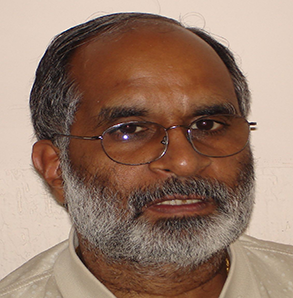
\includegraphics{src/Figures/authors/Rustagi_RPR-PP-Photo.png}} & 

\centerline{\large\bf Prof. Ram P. Rustagi}

\bigskip
Dr.~Ram P. Rustagi is currently working as Professor, CSE dept, KSIT Bangalore, and honed up his academic skills with Ph.D from IIT Delhi, and M.Tech from IISc Bangalore. Prior to KSIT, at Cavisson Systems, he mentored new technology development using Machine Learning techniques in Security and Performance Monitoring. At PES University, he had taught Undergraduates, Post Graduates students, and successfully guided 3 Ph.D scholars. At PESU, he brought innovations in teaching computer network and security courses, and introduced practical experiential learning exercises.\\
&\\  
\raisebox{-3.7cm}{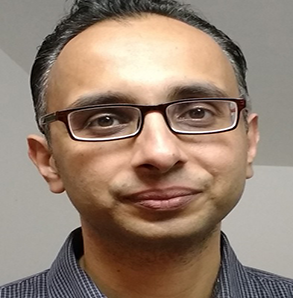
\includegraphics{src/Figures/authors/Viraj_Kumar.png}} & 

\centerline{\large\bf Prof. Viraj Kumar}

\bigskip
Dr.~Viraj Kumar is a Visiting Professor at the Divecha Centre for Climate Change, IISc Bangalore and the Vice-Chair of ACM India’s Special Interest Group in Computer Science Education (iSIGCSE). He was a consultant to the Committee to draft the National Education Policy (2017-18), and contributed to two education-related task groups of the Karnataka Knowledge Commission (2014-16). He holds a PhD in Computer Science from the University of Illinois at Urbana-Champaign.\\
&\\
\clineB{1-2}{2.5}
\end{tabular}

